%template for simulation report

\newpage

\section{Kepler}

\textbf{Object Description:}

\textbf{Simulation Period:} March 2011
% month and year

\textbf{Science Team contact:} Stephen Reynolds

\textbf{NuSIM configuration file:} Kepler.cfg

\textbf{Exposure time:} 100 ks

\textbf{Input Source:} Chandra image with 0.492" pixels.  For the flux used the White Paper numbers F = 6.e-5 (E/10 keV)$^{-3.0}$ ph cm$^{-2}$ s$^{-1}$ keV$^{-1}$.

\textbf{Tiling Method:} Spherical pointing pattern of 9

\textbf{OA Database Version:} 007
% fill in version number e.g. 008

\textbf{Mast Bend Database:} SAA 135
% fill in SAA number

\textbf{Simulation notes:} 
% did we learn anything, did we have to do something special?

\textbf{Status:} 
% are more simulations pending? is it missing something? 

\textbf{Location and name of simulation output:} resource/examples/Kepler in the nusim SVN distribution

\begin{figure}[h]
\begin{center}
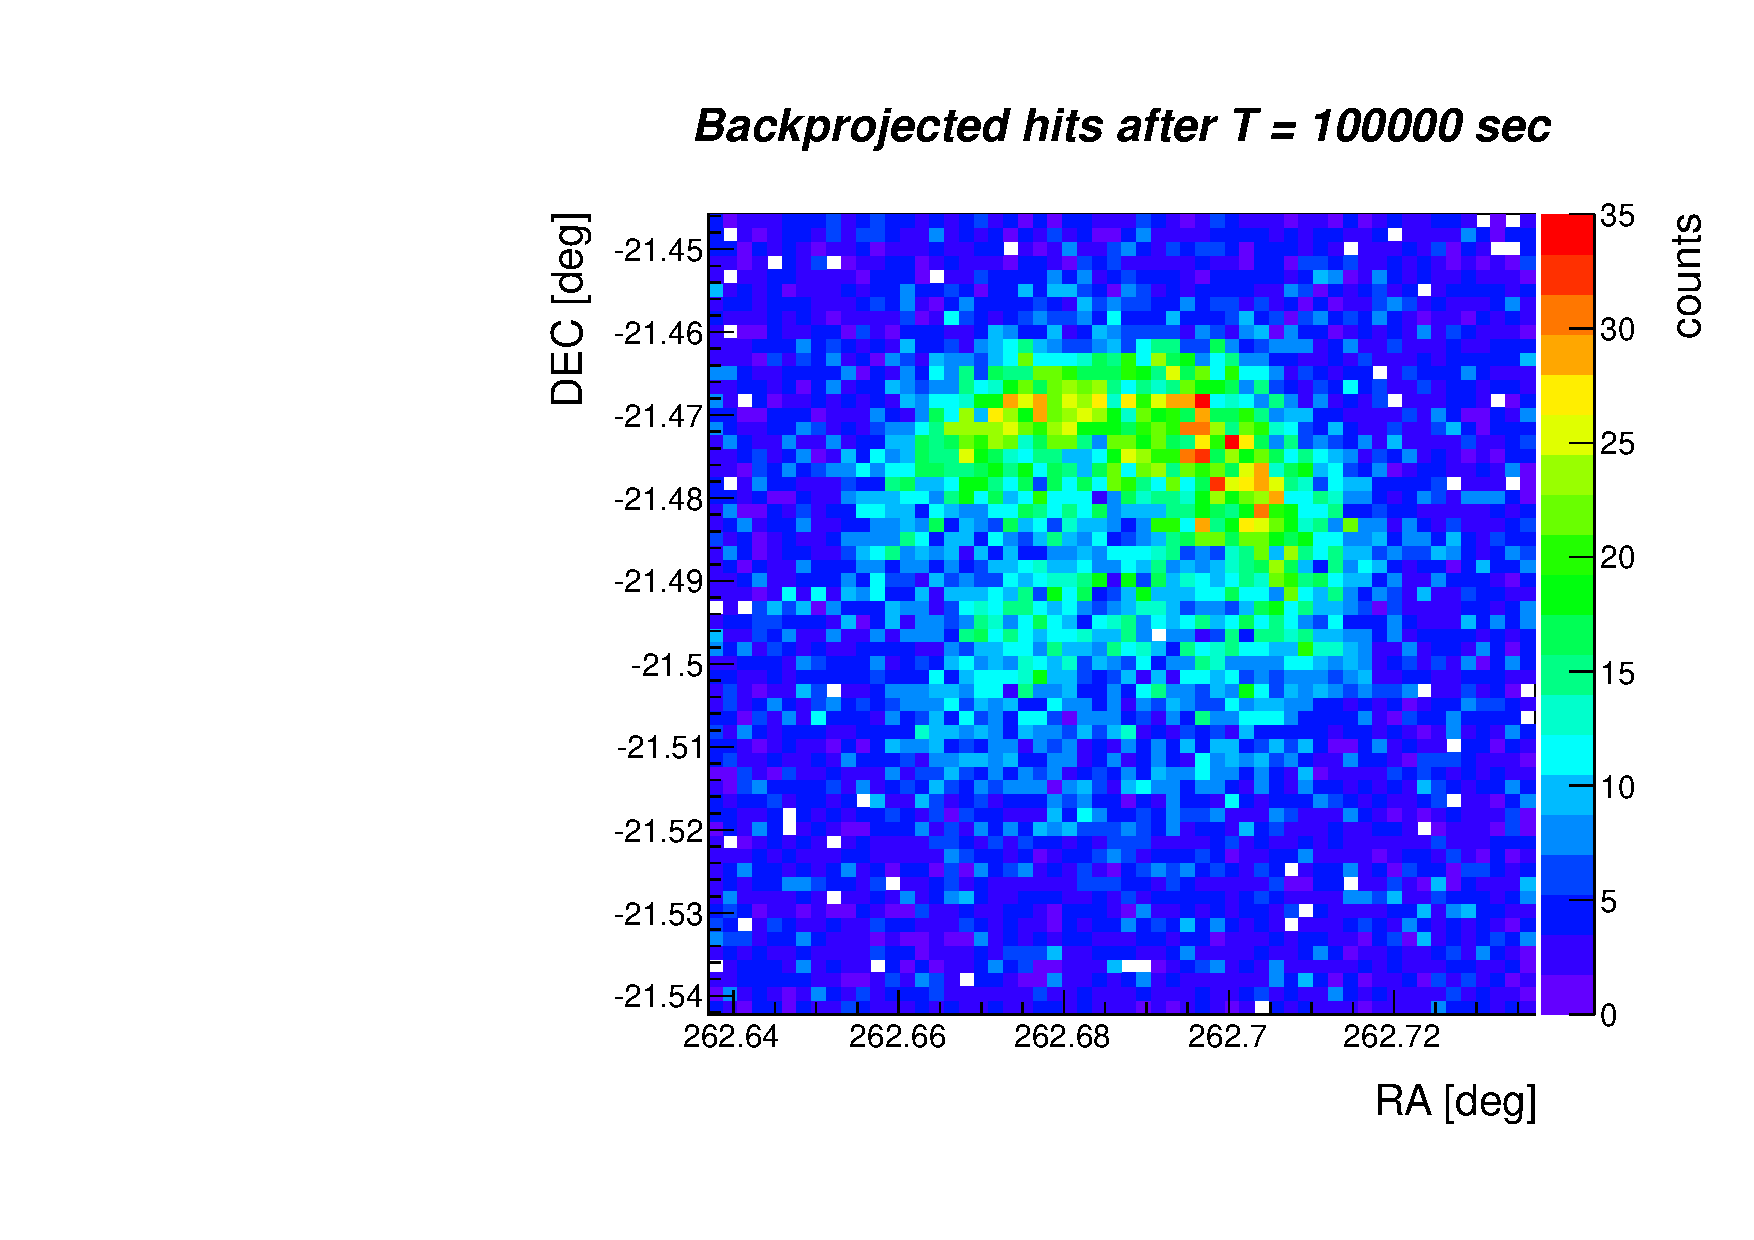
\includegraphics[width=10cm]{Kepler/Kepler.pdf}  % if there is an image put it here  
\caption{Kepler.}
\label{kepler} 
\end{center}
\end{figure}

